\documentclass[11pt]{article}
\usepackage[margin=1.5in]{geometry}
\usepackage{graphicx}
\usepackage{float}
\usepackage{parskip}
\usepackage{amsmath}
\usepackage{pgfplots}
\usepackage{subcaption}
\pgfplotsset{width=10cm, compat=1.9}

\begin{document}

\textbf{\Huge Introduction to Integrals}

Athan Zhang \& Jeffrey Chen

\section{The Area Problem}
Students already know how to find the area of various shapes. However, finding the area of objects and shapes with curved edges is a different problem, and requires a bit more investigation to understand. This so-called "area problem" is the basis for integral calculus and its fundamental concepts.

\subsection{Accumulation of Change}
Finding the area under a curve or function is often important. For example, take the problem below:

Let $r$ represent the rate of snowfall, and $t$ represent time elapsed. How much snow fell in total over the period of time represented on the graph?

\begin{figure}[h]
    \centering
    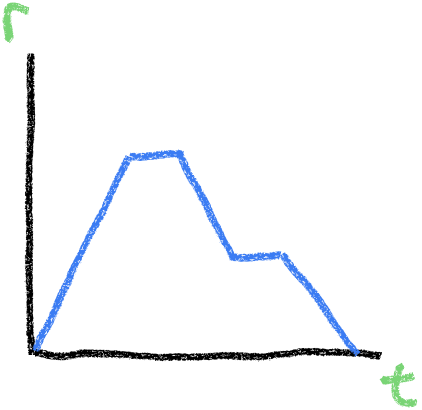
\includegraphics[width=0.3\textwidth]{Calculus/images/snow.png}
\end{figure}


To find the desired quantity here, we must evaluate the area under the function. For functions comprised of line segments such as the one above, this can be achieved by splitting the area up into smaller shapes whose area can then be evaluated using techniques from geometry. 

However, what if the function was a smooth curve instead? Suddenly, with this change, traditional methods cease to work. Instead, we must resort to some more out-of-the-box methods. By splitting the area under the curve into rectangles of equal width, we can approximate the area using the combined area of the rectangles, as shown below:

\begin{figure}[H]
    \centering
    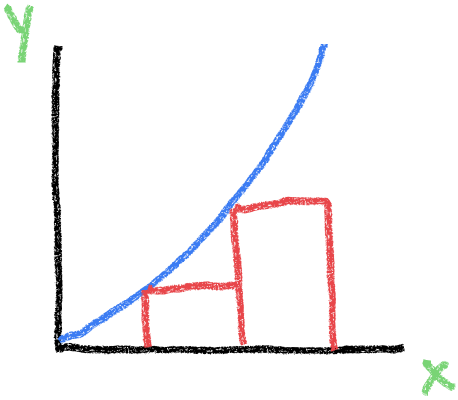
\includegraphics[width=0.3\textwidth]{Calculus/images/2.png}
\end{figure}

Additionally, as we increase the number of rectangles and decrease their width, this approximation becomes more and more accurate, as shown below:

\begin{figure}[H]
    \centering
    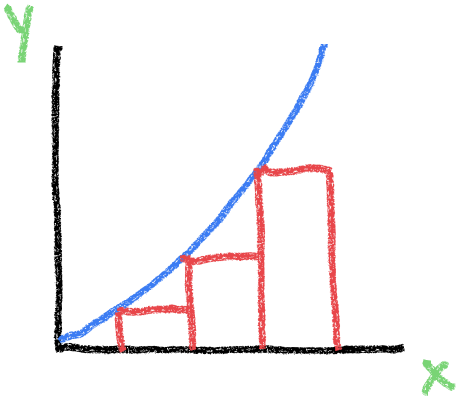
\includegraphics[width=0.3\textwidth]{Calculus/images/3.png}
    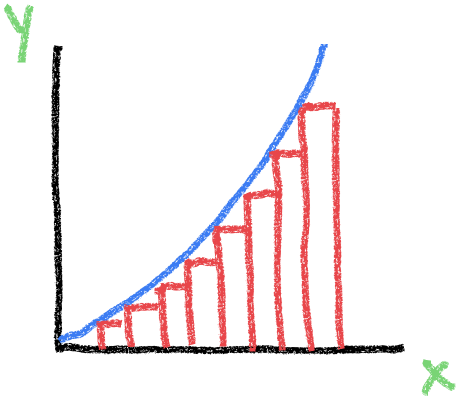
\includegraphics[width=0.3\textwidth]{Calculus/images/more.png}
    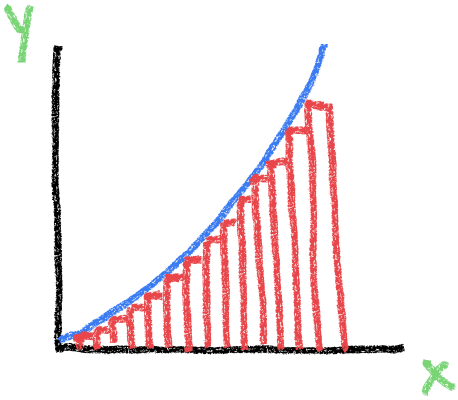
\includegraphics[width=0.3\textwidth]{Calculus/images/many.png}
\end{figure}

\subsection{The Riemann Sum}
This approximation using rectangles is known as the \textbf{Riemann sum}. Let us take a closer look at the mathematics behind the Riemann sum.

Consider a function $f(x)$ defined on the interval $[a, b]$. A Riemann sum utilizing $k$ rectangles splits that interval into $k$ equal subintervals of width $\Delta x$:

\[\Delta x = \frac{b-a}{k} \]

Next, to find the height of the rectangles, we evaluate the value of the function at certain points of each subinterval. The exact point at which we evaluate the function can differ. We may pick the left endpoint of each subinterval, the midpoint, or the right endpoint. Depending on which choice we make, we may refer to our Riemann sum as a \textbf{left hand} Riemann sum, a \textbf{midpoint} Riemann sum, or a \textbf{right hand} Riemann sum, each of which is drawn below.

\begin{figure}[H]
    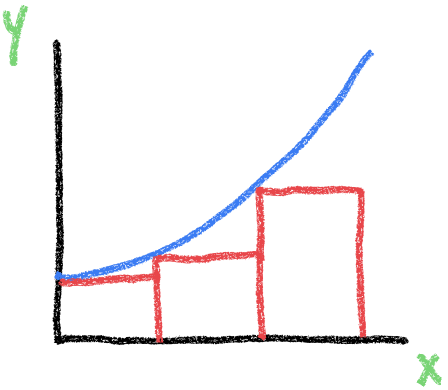
\includegraphics[width=0.3\textwidth]{Calculus/images/left.png}
    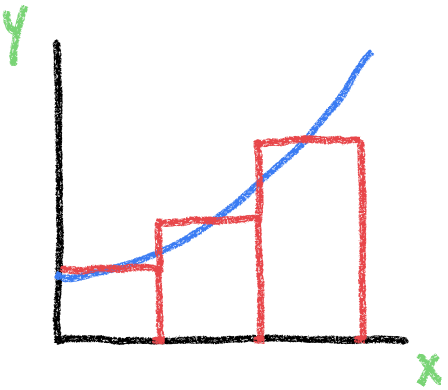
\includegraphics[width=0.3\textwidth]{Calculus/images/midpoint.png}
    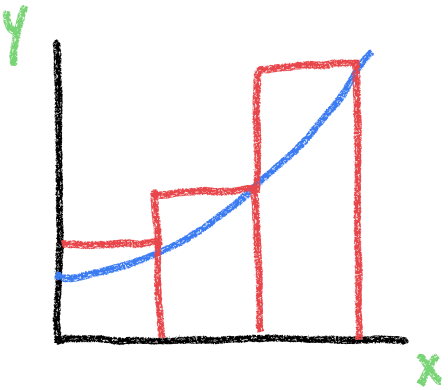
\includegraphics[width=0.3\textwidth]{Calculus/images/right.png}
\end{figure}

Notice that left hand Riemann sums tend to underestimate the area under increasing functions, while right hand Riemann sums tend to overestimate the area. For decreasing functions, this is swapped: left hand Riemann sums tend to overestimate the area, while right hand Riemann sums tend to underestimate the area.

Finally, we can write the formula for a Riemann sum as follows:

\[ A = \sum_{n=1}^{k} f(x_k) \Delta x \]

$k$ represents the number of subintervals/rectangles we plan to divide the area into. Keep in mind the values $x_k$ depend on what type of Riemann sum (left, right, midpoint) we are evaluating.

\subsection{Limit Definition of the Integral}
The \textbf{integral}, one of the two main building blocks of calculus alongside the derivative, simply represents the exact area under a curve. Essentially, the Riemann sum we learned in the last section approximates the value that an integral would give us exactly. The integral representing the exact area under the function $f(x)$ on the interval $[a, b]$ is written as follows:

\[ \int_{a}^{b} f(x) dx \]

The $a$ and $b$ represent the endpoints of the interval, while the $dx$ can be thought of as an infinitesimally small version of $\Delta x$. Notice that due to the Riemann sum becoming infinitely more accurate as we allow $k$ to infinitely increase, we can represent the concept of the integral in the following manner:

\[ \int_{a}^{b} f(x) dx = \lim_{k \to \infty} \sum_{n=1}^{k} f(x_k) \Delta x \]

In other words, the integral can be thought of as a Riemann sum of infinitely many, infinitely thin rectangles. 


\section{Fundamental Theorem of Calculus}
Knowing this limit definition of an integral, it is possible to exactly evaluate the integrals of some simple functions. However, similar to the limit definition of a derivative, it is unwieldy and incredibly time-consuming to do this every time we want to evaluate an integral. 

Luckily, mathematicians of the past discovered a handy relationship between integrals and derivatives that has, over time, helped unite the two concepts into the field of calculus as we know it today. This relationship is known as the first part of a larger concept: the \textbf{Fundamental Theorem of Calculus}.

\subsection{Definite and Indefinite Integrals}
Before moving on, a distinction must be made between two types of integrals. First, the integrals that represent the area under a function for a specific interval, written as the following:

\[ \int_{a}^{b} f(x) dx \]

These integrals are known as \textbf{definite} integrals, and return a number.

However, we can also evaluate integrals with no specified interval, which would instead return a function. These integrals would be written as the following:

\[ \int f(x) dx = \int_{a}^{x} f(t) dt \]

These integrals are known as \textbf{definite integrals}. Students may be reminded of the distinction between general derivatives ($f'(x)$) and derivatives evaluated at a single point ($f'(x_0)$). 

\subsection{First Part}
The first part of the Fundamental Theorem of Calculus, or FTC for short, states the following:


If $f$ is a continuous function defined on an interval $I$, and $a$ is some point in $I$, let $F(x)$ be defined as the following:

\[ F(x) = \int_{a}^{x} f(t) dt \]

Then, the following is true:

\[ F'(x) = f(x) \]

In other words, this establishes an opposite relation between the definite integral and the derivative. For this reason, many refer to the definite integral as the \textbf{antiderivative} This also implies that we can evaluate definite integrals by reversing the processes we used to evaluate derivatives.

\subsection{Second Part}
The second part of the fundamental theorem of calculus relates the definite integral, or antiderivative, with the indefinite integral. It states the following:

If $f$ is a continuous function defined on an interval $I$, and $a$ and $b$ are points in $I$, and $F(x)$ is its antiderivative, then the following is true:

\[ \int_{a}^{b} f(x) dx = F(b) - F(a) \]

This is an extremely important result that connects our two definitions of the integral: definite, a geometric definition involving the area under a curve, and indefinite, an algebraic definition involving the reverse of a derivative.

\section{Evaluating Basic Integrals}

Now that the concept of integrals has been established, we can investigate the process of evaluating them. As stated before, the definite integral or antiderivative of a function can be found by simply reversing the processes we used to find derivatives. Therefore, all of the following are true:

\[ \int af(x) dx = a \int f(x) dx \]
\[ \int (f(x) + g(x)) dx = \int f(x) dx + \int g(x) dx \]
\[ \int x^n dx = nx^{n-1}+C \]
\[ \int \cos(x) dx = \sin(x) + C\]
\[ \int \sin(x) dx = -\cos(x) + C\]
\[ \int e^x dx = e^x + C \]
\[ \int \frac{1}{x} dx = \ln|x| + C \]

Additionally, there is another common integral that is useful to memorize, which we did not cover during the common derivatives section:

\[ \int \frac{1}{x^2+1} dx = \arctan(x) + C \]

There are a few things to note here. 

First, the inclusion of an unknown constant added to the end of each integral once evaluated. This is due to the following observation: each function has only one derivative, but many functions may have the same derivative. Due to the definite integral's nature of being an antiderivative, we must account for this fact.

Second, the absolute value signs around $x$ in the result for the integral of $\frac{1}{x}$. These are necessary due to the fact that $\ln$ is not defined for negative values of $x$.

\subsection{Evaluating Definite Integrals}

Evaluating definite integrals is done using the second part of the FTC. Recall that 

\[ \int_{a}^{b} f(x) dx = F(b) - F(a) \]

First, we must find $F(x)$, which is the antiderivative or definite integral of $f(x)$. This is done through the techniques listed above and below this section. Next, plug in the endpoints of the interval of interest and perform the subtraction to obtain the exact area under $f(x)$.

\section{U-Substitution}
While simple rules like the power rule, constant rule, or addition rule are easy to directly reverse and apply when solving antiderivatives, some of the more useful but complex derivative rules are not. For example, the all-important chain rule allowed us to evaluate derivatives of much more complex functions. We will need a technique similar to the chain rule to evaluate more complex integrals: $u$-substitution.

$u$-substitution can be thought of as performing the chain rule in reverse. Let us start with the chain rule:

\[ \frac{d}{dx}(f(g(x)) = f'(g(x))g'(x) \]

If we integrate this equation and swap the sides, we obtain:

\[ \int f'(g(x))g'(x) dx = f(g(x)) + C \]

Now, it will be useful for us to write $g(x)$ as $u$ instead. Then, the following is true: 

\[ \frac{du}{dx} = g'(x) \]
\[ du = g'(x) dx\]

Then, we can substitute into the previous expression:

\[ \int f'(u)du = f(u) + C \]

This process of simplifying an integral of such form by rewriting part of it as $u$ and making substitutions is called \textbf{u-substitution}. 

Notice that $u$-substitution can be a powerful and efficient tool in simplifying complex integrals into easier ones, but it is not guaranteed to help in every case. Depending on the choice of $u$, as well as the initial integrand, the substitution may not prove to be helpful, and a more useful post-substitution integrand may not be produced. 

In general, there are no set rules for choosing $u$, but the proper intuition will come with experience. It may also be also helpful to think back to the intuition of choosing outer and inner functions for the chain rule.

\section{Integration by Parts}

\subsection{Traditional Method}
Similarly to how $u$-substitution can be thought of as integration's version of the chain rule, \textbf{integration by parts} can be thought of as integration's version of the product rule. In other words, it is a method to deal with integrals of the following form:

\[ \int f(x)g(x) dx \]

To derive the method, we start out with the following expression, assuming $G(x)$ is an antiderivative of $g(x)$.

\[ f(x)G(x) \]

Next, we differentiate this expression using the product rule to obtain the following equation:

\[ \frac{d}{dx}[f(x)G(x)] = f(x)G'(x) + f'(x)G(x)  = f(x)g(x) + f'(x)G(x)\]

From this equation, we know that our original expression, $f(x)G(x)$, is an antiderivative of the final expression on the right hand side of the equation. In other words:

\[ \int [f(x)g(x) + f'(x)G(x)] dx = f(x)G(x) \]

Due to the addition rule of integrals, we can split the integral on the left hand side into two separate ones:

\[ \int[f(x)g(x)]dx + \int[f'(x)G(x)]dx = f(x)G(x) \]

Finally, we can isolate our desired integral:

\[ \int[f(x)g(x)]dx = f(x)G(x) - \int[f'(x)G(x)]dx \]

This formula effectively converts the problem of integrating $\int[f(x)g(x)]dx$ into the problem of integrating $\int[f'(x)G(x)]dx$, which in many cases is much simpler. 

We can make the formula cleaner and easier to understand by rewriting a few variables. Let 

\[ u = f(x) \]
\[ v = G(x) \]

Then, the following is true:

\[ du = f'(x)dx \]
\[ dv = g(x)dx \]

We can substitute these variables into our integration by parts formula to obtain:

\[ \int u dv = uv - \int v du\]

Just like $u$-substitution, the art of choosing which parts of the integrand are $u$ and $dv$ respectively is a skill which requires experience and intuition to perfect, and there are no hard rules when doing so. However, a general guideline to follow is this: in most cases, a function that becomes simpler when differentiated is the best choice for $u$. Also, when functions such as $\sin x$ or $\cos x$ or $e^x$ appear, they are generally not a good choice for $u$, and therefore are a good choice for $dv$, because their nature does not change when differentiated. 

\subsubsection*{Example 1}
\[ \int x \cos x dx\]

We will choose $x$ to be our $u$, as it gets simpler when differentiated. Then, $\cos x$ will be our $dv$. 

\[ u = x \to du = dx \]
\[ dv = \cos x dx \to v = \sin x \]

We can now put together our integration by parts formula:

\[ \int x \cos x dx = uv - \int v du = x \sin x - \int \sin x dx = x \sin x + \cos x \,\,(+C)\]
% x cos x
% x^3 e^x

\subsubsection*{Example 2}
However, note that not all applications of integration by parts are as quick or easy as the one shown above. Sometimes, just as we may have needed to apply product rule multiple times to obtain a derivative in the past, we may need to apply integration by parts multiple times to obtain an integral.

\[ \int x^3 e^x dx \]

We will choose $x^3$ to be our $u$, as it gets simpler when differentiated, while $e^x$ stays the same. Then, 

\[ u = x^3 \to du = 3x^2 dx \]
\[ dv = e^x dx \to v = e^x \]

We can now put together our integration by parts formula:

\[ \int x^3 e^x dx = uv - \int v du = x^3e^x - \int e^x (3x^2 dx)\]

As you can see, we have converted the problem of integrating $\int x^3 e^x dx$ into the problem of integrating $\int 3x^2e^x dx$. However, this new integral still requires another application of integration by parts to solve:

\[ u = 3x^2 \to du = 6x dx \]
\[ dv = e^x dx \to v = e^x \]

Apply integration by parts to obtain:

\[ \int 3x^2e^x dx = 3x^2e^x - \int e^x(6x dx)\]

We can substitute this into our previous expression to obtain:

\[ \int x^3 e^x dx = x^3e^x - (3x^2e^x - \int e^x(6x dx))\]
\[ = x^3e^x - 3x^2e^x + \int 6xe^x dx\]

Note that the new integral of interest, $\int 6xe^x dx$, requires yet another application of integration by parts:

\[ u = 6x \to du = 6 dx\]
\[ dv = e^x dx \to v = e^x\]

Apply the formula to get:

\[ \int 6xe^xdx = 6xe^x - \int e^x(6 dx)\]

Substitute into the original expression to get:

\[ \int x^3 e^x dx = x^3e^x - 3x^2e^x + (6xe^x - \int 6e^x dx)\]
\[ = x^3e^x - 3x^2e^x + 6xe^x - 6e^x \,\,(+C)\]

As can be seen, this was a long process which required a total of three applications of integration by parts. This should show that organization of work and clarity of mind are important when performing such tasks.

\subsection{Table Method}
Aside from the traditional method of designating $u$ and $dv$ functions from a given integrand, there is another slightly different method of performing integration by parts. At its core, this method achieves the same thing through the same process, but through the way it is set up and organized, it is advantageous in some cases, such as repeated integration by parts.

This method is known as the \textbf{table method} of integration by parts. The first step is to split the integrand into two parts, similar to before, one of which will be differentiated and one of which will be integrated. 

Next, we construct a table with three columns, the leftmost column containing alternating + and - signs, the middle column containing the part to be differentiated, and the rightmost column containing the part to be integrated. 

Next, we repeatedly differentiate the middle column and integrate the right column. In easy cases, the middle column will eventually reach zero, and that is our sign to stop. However, sometimes this will not be the case. In these cases, we may choose where to stop, and the final product would be done horizontally under an integral. See the example in the next section for clarification on what this means.

Finally, we multiply the middle and rightmost columns diagonally and add according to sign. 

\subsubsection*{Example 1}

\[ \int x \cos x dx\]

We split the integrand into $x$ and $\cos x$. Because $x$ gets simpler as we differentiate it, we put it in the middle, or "to be differentiated" column. The $\cos x$ gets put in the rightmost column.

\begin{table}[H]
    \centering
    \begin{tabular}{c|c|c}
        sign & d & I \\
        \hline
        + & $x$ & $\cos x$ \\
        - & $1$ & $\sin x$\\
        + & $0$ & $-\cos x$ 
    \end{tabular}
\end{table}

Finally, we take each nonzero entry in the derivatives column, multiply it by the entry in the integrals column that is diagonally down and to the right, and add according to sign. This would yield:

\[ \int x \cos x dx = (x)(\sin x) - (1)(-\cos x) = x\sin x + \cos x \,\, (+C)\]

\subsubsection*{Example 2}
Now, let us investigate a case where the table method is more advantageous to use than the traditional method: repeated integration by parts.

\[ \int x^3 e^x dx \]

We will split the integrand into $x^3$ and $e^x$. $x^3$ will eventually get simpler and reach zero as we differentiate it repeatedly, so we will put it in the middle column. We construct our table as follows: 

\begin{table}[H]
    \centering
    \begin{tabular}{c|c|c}
        sign & d & I \\
        \hline
        + & $x^3$ & $e^x$ \\
        - & $3x^2$ & $e^x$\\
        + & $6x$ & $e^x$ \\
        - & $6$ & $e^x$ \\
        + & $0$ & $e^x$ \\
    \end{tabular}
\end{table}

Finally, we can add our products together: 

\[ \int x^3e^x dx = (x^3)(e^x) - (3x^2)(e^x) + (6x)(e^x) - (6)(e^x) \]
\[ = x^3e^x - 3x^2e^x + 6xe^x - 6e^x \,\, (+C)\]

As seen before, this same integral required much more thought and work when using the traditional method, but when using the table method, its organization allows us to perform the repeated integration by parts much more efficiently and neatly.

\subsection{Cyclic Integrations by Parts}
% cyclic integrations
In some complicated cases, even if we do many layers of integration by parts, the integral of interest never becomes easier to do. If this is true, the integral may be impossible to solve with traditional basic methods. 

However, in some even more peculiar cases, integration by parts may work, albeit with a little more out-of-the-box thinking. This occurs when repeated integration by parts can eventually change the integral of interest back into the original integral, and it can be solved for like an equation. These peculiar cases can be thought of as \textbf{cyclic} integrations by parts. An example will be shown to further illustrate the meaning of this.

\subsubsection*{Example}
\[ \int e^{2x}\cos x dx \]
If we separate our integrand and construct our table, we can obtain the following:

\begin{table}[H]
    \centering
    \begin{tabular}{c|c|c}
        sign & d & I \\
        \hline
        + & $e^{2x}$ & $\cos x$ \\
        - & $2e^{2x}$ & $\sin x$\\
        + & $4e^{2x}$ & $- \cos x$ 
    \end{tabular}
\end{table}

Following our table rules listed at the beginning of the previous section, we have the following: 

\[ \int e^{2x}\cos x dx = e^{2x}\sin x - 2e^{2x}(-\cos x) + \int 4e^{2x}(-\cos x) dx\]

(Note that, due to the nonconvergence to zero of the derivative column, we must cut off the table at some point and add the integral of the horizontal product of the final entries, as detailed at the beginning of the previous section.)

Now, we can simplify to the following:

\[ \int e^{2x}\cos x dx = e^{2x}\sin x + 2e^{2x}\cos x - 4\int e^{2x}\cos x dx\]

We can now see that after exactly two applications of integration by parts, the new integral of interest is the same as the original integral. Therefore, we can isolate the like terms on one side and solve like an equation:

\[ 5 \int e^{2x}\cos x dx = e^{2x}\sin x + 2e^{2x}\cos x \]
\[ \int e^{2x}\cos x dx = \frac{e^{2x}\sin x + 2e^{2x}\cos x}{5}\]

These scenarios take a bit of intuition to recognize, but are relatively simple once they are grasped. Note that the product of any two of the functions $\sin x$, $\cos x$, and $e^x$ can result in cyclic cases like this due to the nature of their derivatives.

\end{document}
